\documentclass{article}

% if you need to pass options to natbib, use, e.g.:
\PassOptionsToPackage{numbers, square}{natbib}
% before loading neurips_2022

% ready for submission
\usepackage[preprint]{neurips_2022}

% to compile a preprint version, e.g., for submission to arXiv, add add the
% [preprint] option:
% \usepackage[preprint]{neurips_2022}

% to compile a camera-ready version, add the [final] option, e.g.:
%     \usepackage[final]{neurips_2022}

% to avoid loading the natbib package, add option nonatbib:
% \usepackage[nonatbib]{neurips_2022}

\usepackage[utf8]{inputenc} % allow utf-8 input
\usepackage[T1]{fontenc}    % use 8-bit T1 fonts
\usepackage{hyperref}       % hyperlinks
\usepackage{url}            % simple URL typesetting
\usepackage{booktabs}       % professional-quality tables
\usepackage{amsmath,amsthm,amsfonts,amssymb}       % blackboard math symbols
\usepackage{nicefrac}       % compact symbols for 1/2, etc.
\usepackage{microtype}      % microtypography
\usepackage{xcolor}         % colors
\usepackage{graphicx}
\usepackage{float}
\usepackage{algpseudocode}
\usepackage{algorithm}
\usepackage[capitalise]{cleveref}
\usepackage{caption, subcaption}
\algnewcommand\algorithmicforeach{\textbf{for each}}
\algdef{S}[FOR]{ForEach}[1]{\algorithmicforeach\ #1\ \algorithmicdo}

% \usepackage{parskip}
\graphicspath{{../plots/}}

\title{Q Learning and Deep Q Network}

\author{%
      Ling Fei Zhang\\
      Department of Computer Science\\ McGill University\\ Montreal, QC \\
      \texttt{lzhang133@gmail.com} \\
}

\begin{document}
\maketitle

\begin{abstract}
      In this paper, we compare two widely used RL algorithms, Q Learning and Deep Q Network (DQN), in the context of two games, CartPole and Lunar Lander. Our results demonstrate that DQN learns faster than Q Learning, but can be more unstable during the learning process. In constrast, Q Learning leanrs more steadily but at a slower rate. These findings usggest that the choice of the algorithm depends on the specific application and trade-offs between speed and stability. Our work contributes to the understanding of the performance characteristics of Q Learning and DQN, and can help guide the selection of RL algorithms for similar tasks in the future.
\end{abstract}

\section{Introduction}

Reinforcement learning is a subset of artificial intelligence that concerns
itself with developing agents that can learn to take actions in a stochastic
environment with the goal to maximize a reward function. In recent years,
reinforcement learning has gained considerable attention as it is a powerful
approach that can be used in a wide range of applications, from robotics and
gaming to finance and healthcare. Among the many algorithms in reinforcement
learning, Q Learning has been one of the most popular and most used. However, Q
Learning also has its limitations when it comes to handling large state spaces
and continuous action spaces. To solve this problem, significant progress has
been made by exploting the advantages of deep learning in reinforcement
learning, resulting in the ``Deep Q Network (DQN)'' algorithm
\cite{DBLP:journals/corr/MnihKSGAWR13}. DQN combines Q Learning with deep
neural networks to learn policies that can handle complexe state-action spaces.

Q Learning is a model free reinforcement learning algorithm that uses a table
to store the Q values for each state-action pair. The Q value repreesnts the
expected return that the agent can obtain by taking a specific action in a
given state. To learn, Q Learning updates the Q values based on the Bellman
equation. To be more specific, the algorithm learns by updating the expected
return in terms of the immediate reward and the expected return in the next
state. In simple environments, Q Learning is very effective. However, the model
struggle in more complex environments, usually due to the high dimensionality.
This is known as the curse of dimensionality, where the number of actions
increases exponentialy with the number of degrees of freedom
\cite{soft_update}, making it impractical to store and update the Q values for
all the state-action pairs.

To overcome the limitations of Q Learning, DQN was introduced. DQN combines Q
Learning with deep neural networks to learn policies that can handle
state-action spaces. The deep neural network approximates the Q values, which
enables the agent to learn a function that maps the states to the Q values.
Using neural networks as our function approximator, we can handle large state
spaces as well as continuous action spaces.

However, no algorithm is perfect, as DQN faces its own challenge of
instability. In fact, DQN can be quite unstable during the learning process and
also requires careful hyperparameter tuning. The instability arises mainly from
the non-stationarity of the learning process, where the Q values change as the
agent learns, which then affects the target values used in the update rule. The
need of careful tuning of hyperparameters arises from the complexity of the DQN
algorithm, which involves the use of mutilple layers of neural networks,
different learning rates and replay buffers.

% In this project, the aim is to compare the performance of Q Learning and DQN in
% two games and observe the advantages and limitations of each algorithm. By
% comparing the results, we hope to gain insights into the strenghts and
% weaknesses of each algorithm and provide a better understanding of their
% performance in different environments. The motivation for this comparison comes
% from the need to understand the trade-offs between the two algorithms and their
% applicability in different scenarios.

\section{Background}

In this project, we will compare the performance of Q Learning and DQN
algorithms on two games from the OpenAI Gym environment: CartPole and Lunar
Lander. CartPole is a game that involves balancing a pole on a cart by moving
the cart left or right. On the other hand, Lunar Lander is a game that involves
landing a spacecraft on a landing pad by controlling its thrusters. Both games
have discrete action spaces, which make them suitable for testing the
performance of Q Learning and DQN.

\section{Methodology}
\subsection{Q Learning}
The idea of Q Learning is to select an action given a particular state from a
function \(Q\), which the agent in turns receives an reward and a next state.
The agent then updates \(Q\) in respect to maximizing the long term expected
sum of rewards. The core of the Q Learning algorithm is defined by the update
rule as follows
\begin{equation}
      Q(s_t, a_t) = Q(s_t, a_t) + \alpha \left[r_{t+1} + \gamma \max_{a} Q(s_{t+1}, a) - Q(s_t, a_t)\right]
      \label{eq:q_update_rule}
\end{equation}

In this case, the learned action-value function \(Q\) directly approximates
\(q_*\), the optimal action-value function, independent of the policy being
followed. As a result, this drastically simplifies the analysis of the
algorithm. As it turns out, all that is required for proper convergence is that
all state-action pairs continue to be updated\cite{sutton}.

Q Learning's algorithm uses a table to store the Q values for each of the
state-acion pairs, and its limitation lies on the dimensionality of the state
space. In fact, since both the CartPole and Lunar Lander games have continuous
observation space, it is practically impossible to store the Q values for all
state-action pairs. Thus, we must first discretize the continuous states into
discrete states \cite{discretization}. This can be done by taking the range of
values for each feature of the state, and dividing the range into a specified
number of bins. In the case that a feature has unlimited range (i.e. min =
\(-\infty\) and max = \(\infty\)), we can set a minimum and maximum manually
based on the observations. For example, in CartPole, the cart velocity and the
pole angular velocity are unbounded. However, from the observations, we decided
that a minimum of -3.5 and a maximum of 3.5 is a good range for the cart
velocity. To train our agent, we simply pass the required arguments to the
\verb+Agent_Q+ class, and train it on a desired number of episodes. In our
case, we number of training episodes is 500 for both games.

We used very similar hyperparameters for both games, with the exception of the
learning rate. In particular, for both games, we used a discount factor of
0.99, a start epsilon of 1, a minimum epsilon of 0.01, a discretization done by
dividing the range of a feature into 10 equal sized bins
\cite{discretization_tech}, and an epsilon linear decay with a slope of
\(5^{-4}\). With some experimentation, we discovered that the best learning
rates for CartPole and Lunar Lander are 0.25 and 0.005 respectively.

\subsection{DQN}
To build our agent for DQN, a few steps are necessary as we need a deep neural
network to approximate our Q values. Since DQN is a off policy reinforcement
learning algorithm, it uses a technique called experience replay. Thus, our
first step is to implement \verb+ReplayMemory+, which acts as a replay buffer
of past experiences. Each memory consist of a 5-tuple, namely (state, action,
reward, next state, done). We also implemented the \verb+sample+ method since
the algorithm learns by sampling from the buffer, and updates the Q network
accordingly.

Next, we implemented the deep neural network, which consists of two hidden
layers, each with a default number of 128 units. We used \verb+ReLU+ activation
function, \verb+Adam+'s optimizer and calculated our loss with
\verb+SmoothL1Loss+. We decided to use the Huber loss during our implementation
to make our agent more robust to outliers when the estimates of Q values are
noisy. In fact, the Huber loss acts like the mean squarred error when the error
is small, and acts like the mean absolute error when it's large \cite{hubert}.
We used In the \verb+forward+ method, our network takes in a state, and outputs
a Tensor of shape \verb+action_space+, each element corresponding to the Q
value of the state-action pair.

With this, we can build our RL agent. We built the agent with both a policy as
well as a target network in order to make learning more stable. For our
experiment, we initialized a replay buffer of size 100000, and trained our
agent for 500 episodes. The actions are sampled based on an epsilon-greedy
exploration. The full algorithm of DQN is described in \cref{alg:dqn}.

Unlike Q Learning, DQN does not need to discretize the states of a continuous
observation space. This is because the continuous features can be passed
directly into the deep neural network, and obtain the state-action Q values as
outputs. However, DQN is computationally expensive compared to Q Learning,
since we are working with two neural networks and performing gradient descent.

We used the same hyperparameters for both games. Specifically, we used a
learning rate of 0.003, a discount factor of 0.99, an initial epsilon of 1, a
minimum epsilon of 0.01, an epsilon decay of \(5^{-4}\), a tau of 0.005 and a
batch size of 64.

\section{Algorithm}

\subsection{Q Learning}

\begin{algorithm}[H]
      \caption{Q Learning(episodes, \(\alpha, \epsilon, \gamma\))}
      \label{alg:qlearning}
      \begin{algorithmic}[1]
            \State Initialize \(Q(s,a)\) for all \(s \in \mathcal{S}, a \in \mathcal{A}(s)\) arbitrarily.
            \State Set \(Q(terminal, \cdot) = 0 \) for all terminal states.
            \ForEach {episode in episodes}
            \State Initialize \(s\)
            \State done \(\leftarrow\) False
            \While {not done}
            \State Choose \(a \in \mathcal{A}\) from \(s\) using policy derived from \(Q\) \Comment{\(\epsilon\)-greedy, Softmax}
            \State Take action \(a\)
            \State Observe reward \(r\) and next state \(s'\)
            \State \(Q(s, a) \leftarrow Q(s, a) + \alpha \left[r + \gamma \max_{a} Q(s', a) - Q(s, a)\right]\) \Comment{\cref{eq:q_update_rule}}
            \State \(s \leftarrow s'\)
            \EndWhile
            \EndFor
      \end{algorithmic}
\end{algorithm}

In \cref{alg:qlearning}, \(\alpha\) is the learning rate, \(0 < \gamma \leq 1\)
is the discount factor, and \(\epsilon\) is the exploration factor for the
agent.

\subsection{Deep Q Network}

\begin{algorithm}[H]
      \caption{DQN(episodes, \(\alpha, \epsilon, \gamma, C\))}
      \label{alg:dqn}
      \begin{algorithmic}[1]
            \State Initialize replay buffer \(\mathcal{D}\) with maximum capacity 100000
            \State Initialize policy network \(Q\) with random weights \(\theta\)
            \State Initialize target network \(\tilde{Q}\) with random weights \(\tilde{\theta}\) \Comment{more stable learning}
            \ForEach{episode in episodes}
            \State Initialize \(s\)
            \State Set \(t \leftarrow 0\) \Comment{time step}
            \State \(done\) \(\leftarrow\) False
            \While {not \(done\)}
            \State Choose \(a \in \mathcal{A}\) from \(s\) using policy network \(Q\) \Comment{\(\epsilon\)-greedy, Softmax}
            \State Take action \(a\)
            \State Observe reward \(r\), next state \(s'\) and \(done\)
            \State Store transition \((s, a, r, s', done)\)
            \State Sample a minibatch of random transitions \((s, a, r, s', done)\) from \(\mathcal{D}\)
            \State Set \(\hat{y} =
            \begin{cases}
                  r                                                  & \quad \text{if }s \text{ is a terminal state} \\
                  r + \gamma \max_a \title{Q}(s', a; \tilde{\theta}) & \quad \text{otherwise}
            \end{cases}\) \Comment{use target network}
            \State Perform a gradient descent step on \(\left(\hat{y} - Q(s, a; \theta)\right)^2\) with respect to the policy network parameters \(\theta\)
            \If {\(t \text{ mod } C = 0\)}
            \State \(\tilde{Q} \leftarrow Q\) \Comment{resets target network}
            \EndIf
            \State C \(\leftarrow\) C + 1
            \EndWhile
            \EndFor
      \end{algorithmic}
\end{algorithm}

\section{Results}

After training both agents for 500 episodes, we can observe the training return
for both agents in \cref{fig:train}.

\begin{figure}[H]
      \centering
      \begin{subfigure}[H]{0.49\textwidth}
            \centering
            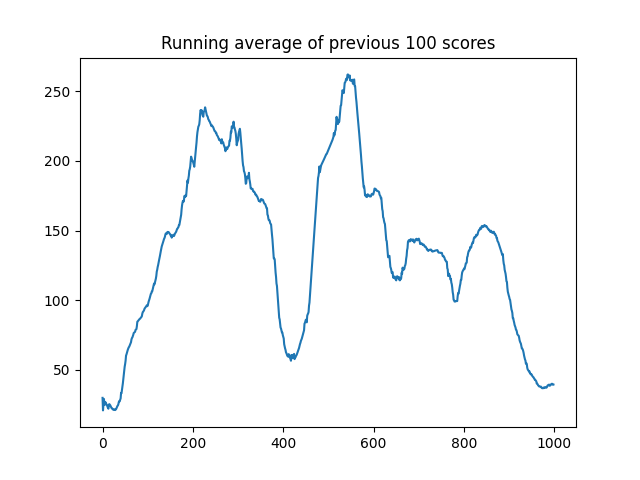
\includegraphics[width=\textwidth]{cartpole}
            \caption{Q Learning vs DQN in CartPole}
            \label{fig:cartpole}
      \end{subfigure}
      \begin{subfigure}[H]{0.49\textwidth}
            \centering
            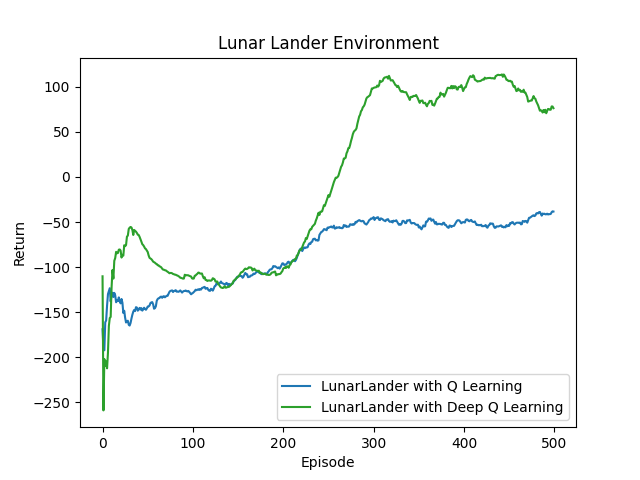
\includegraphics[width=\textwidth]{lunar}
            \caption{Q Learning vs DQN in Lunar Lander}
            \label{fig:lunar}
      \end{subfigure}
      \caption{500 training episodes for Q Learning and DQN. Returns are averaged over the last 100 episodes.}
      \label{fig:train}
\end{figure}

Immediately, we notice a significant learning improvement in DQN over Q
learning in both games.

\subsection{CartPole}
In the CartPole environment, we can see that DQN easily reached an average
return of 300 shortly after 300 training episodes. We also observe a big drop
in average return after approximately 350 episodes. We suspect that this comes
from the fact that the agent escaped a local minima, and tries to work its way
to a global minima as the return peaks upwards again at around episode 450. We
can see that DQN's return grows quickly, but also much more unstably to Q
Learning. This is a direct consequence of the algorithm, as one of its
limitations is the instability during the learning process.

As for Q Learning, we can see that the agent learns at a much slower but more
steady rate compared to DQN. We can see that even after 500 episodes of Q
Learning training, the agent seems to only obtain an average return of a little
less than 100. This could be that the agent is stuck in a local minima. Due to
the good returns, the agent might decide to stay in the local minima, rather
than risking to espace it.

\subsection{Lunar Lander}
In the Lunar Lander environment, we can once more see that DQN out performs Q
Learning. Once more, we can see the properties of each algorithm. Clearly,
DQN's learning is fast but unstable. The agent reaches a return of -50 at
episode 50, but it decreases to approximately -125 at episode 150. Then, the
agent seems to have learnt some important information, as the return spikes up
to +100 shortly after. It then once more comes to a plateau for the remaining
of the training episodes.

On the other hand, Q Learning has a slower but stable learning. The agent
doesn't have any drastic change in average returns. Rather, the average return
slowly increases.

\section{Conclusion}
This in paper, we have studied two popular reinforcement learning algorithms, Q
Learning and DQN, on two different games, CartPole and Lunar Lander. Our
results showed that DQN was able to learn faster in both games, but it
exhibited some instability during the learning process. In constrast, Q
Learning learned more steadily but at a slower pace. These findings suggest
that the choice of algorithm depends on the specific application and trade-offs
between speed and stability.

As a future direction, we suggest exploring modifications of Deep Q Learning,
such as deep deterministic policy gradient (DDPG), which combines Q Learning
with policy gradients to learn a deterministic policy directly. This approach
has been shown to be effective in continuous action spaces and could
potentially address some of the instability issues observed in DQN. Overall,
our work highlights the importance of carefully selecting the appriopriate
reinforcement learning algorithm for a given task.

\newpage
\nocite{*}
\bibliographystyle{plain}
\bibliography{References}

\end{document}